
% Basic setup. Most papers should leave these options alone.
\documentclass[a4paper,fleqn,usenatbib]{../mnras}

\usepackage{newtxtext,newtxmath}

% Use vector fonts, so it zooms properly in on-screen viewing software
% Don't change these lines unless you know what you are doing
\usepackage[T1]{fontenc}
\usepackage{ae,aecompl}


%%%%% PACKAGES %%%%%

% Only include extra packages if you really need them. Common packages are:
\usepackage{graphicx}	% Including figure files
\usepackage{amsmath}	% Advanced maths commands
\usepackage{amssymb}	% Extra maths symbols
\usepackage{color}

%%%%% CUSTOM COMMANDS %%%%%

\newcommand{\Nant}{\ensuremath{N_{\mathrm{ant}}}}
\newcommand{\Ng}{\ensuremath{N_{\mathrm{g}}}}
\newcommand{\s}{\ensuremath{\hat{\mathbf{s}}}} % s-hat for sine-projected direction
\newcommand{\spix}{\ensuremath{\hat{\mathbf{s}}_{\mathrm{pix}}}}
\newcommand{\Cna}[1][n]{\ensuremath{\mathcal{C}^{(#1)}_{a,\spix}}}
\newcommand{\ri}{\ensuremath{\mathbf{r}_i}}
\newcommand{\ra}{\ensuremath{\mathbf{r}_a}}
\newcommand{\rb}{\ensuremath{\mathbf{r}_b}}
\newcommand{\beamr}{\ensuremath{\widetilde{W}}}
\newcommand{\beamtheta}{\ensuremath{W}}
\newcommand{\Er}[1]{\ensuremath{\widetilde{E}_{#1}}}
\newcommand{\Erest}[1]{\ensuremath{\hat{\widetilde{E}}_{#1}}}
\newcommand{\V}{\ensuremath{\widetilde{V}}}
\newcommand{\dif}{\mathrm{d}}
\newcommand{\caliter}{50}
\newcommand{\damp}{\ensuremath{\Delta}}
\newcommand{\itr}{20}

%%%%%%%%%%%%%%%%%%% TITLE PAGE %%%%%%%%%%%%%%%%%%%

% Title of the paper, and the short title which is used in the headers.
% Keep the title short and informative.
\title[E-field Parallel Imaging Calibration]{An Efficient E-field Parallel Imaging Calibration Algorithm for Next-Generation Radio Telescopes}

% The list of authors, and the short list which is used in the headers.
% If you need two or more lines of authors, add an extra line using \newauthor
\author[Beardsley et al.]{
Adam P. Beardsley,$^{1}$\thanks{E-mail: Adam.Beardsley@asu.edu}
Nithyanandan Thyagarajan,$^{1}$
Judd D. Bowman$^{1}$
\newauthor
and Miguel F. Morales$^{2}$
\\
% List of institutions
$^{1}$Arizona State University, School of Earth and Space Exploration, Tempe, AZ 85287, USA\\
$^{2}$University of Washington, Department of Physics, Seattle, WA 98195, USA\\
}

% These dates will be filled out by the publisher
\date{Accepted XXX. Received YYY; in original form ZZZ}

% Enter the current year, for the copyright statements etc.
\pubyear{2015}

% Don't change these lines
\begin{document}
\label{firstpage}
\pagerange{\pageref{firstpage}--\pageref{lastpage}}
\maketitle

% Abstract of the paper
\begin{abstract}
Abstract here (250 words)
\end{abstract}

\begin{keywords}
instrumentation: interferometers -- techniques: image processing -- techniques: interferometric
\end{keywords}


%%%%%%%%%%%%%%%%% BODY OF PAPER %%%%%%%%%%%%%%%%%%

\section{Introduction}
In order to satisfy the survey speeds required for precision cosmology as well as searches for fast radio transients, radio astronomy is undergoing a paradigm shift toward interferometers consisting of hundreds to thousands of small, widefield antennas. Many arrays with this design are already built or under construction including the Hydrogen Epoch of Reionization Array\footnote{http://reionization.org} (HERA), the Murchison Widefield Array (MWA;\citealt{tin13,bow13}), the Precision Array for Probing the Epoch of Reionization (PAPER; \citealt{par10}), the LOw Frequency ARray (LOFAR;\citealt{van13}), the Canadian Hydrogen Intensity Mapping Experiment (CHIME,\citealt{ban14}), the Long Wavelength Array (LWA, \citealt{ell13}), and the low frequency Square Kilometer Array (SKA1-Low \citealt{mel13}).

Traditional radio correlators cross-multiply the voltage signals from all pairs of antennas, and the computation scales as the number of antennas squared, $\mathcal{O}(\Nant^2)$ \citep{bun04}. As the number of elements in future arrays grows, the computational cost will become prohibitively expensive, and exploring efficient correlator schemes is essential to enable next generation instruments \citep{lon00}. Meanwhile, radio transient monitoring requires access to high time and frequency resolution data. For example, Fast Radio Bursts (FRBs) are highly unexplored at low frequencies (< 1 GHz), but are expected to occur on timescales $\Delta t \sim$ 1--10~ms \citep{tho13}. Recording the full visibility matrix for $\Nant \gtrsim 10^3$ arrays at this timescale leads to extremely high data write rates. 

Direct imaging correlators are a new variety of radio correlator which aim to alleviate both the computational strain of forming $\Nant^2$ correlations and the high data throughput associated with short timescale science. This is done by performing a spatial fast Fourier transform (FFT) to image the antenna voltages, then squaring and averaging in time. This process scales as $\mathcal{O}(\Ng \log_2 \Ng)$, where \Ng~is the number of grid points in the FFT \citep{mor11, teg09, teg10}. For certain classes of telescopes, significantly those envisioned for next generation cosmology experiments, this scaling is a large improvement over the $\Nant^2$ scaling of traditional methods. Furthermore, because images are generated online, the native output bandwidth will be lowered (assuming $\Ng < \Nant^2$), and has the potential to be lowered even further with online transient processing.

A handful of prototype direct imaging correlators have been tested on arrays including the Basic Element for SKA Training II (BEST-2) array \citep{fos14}, the Omniscope \citep{zhe14}, and an earlier pulsar timing experiment at GHz frequencies \citep{oto94, dai00}. Each of these are examples of so-called FFT correlators -- a subclass of direct imaging correlators which rely on identical antennas with restricted placement, which allows the FFT to be performed without gridding. We recently released the E-field Parallel Imaging Correlator \citep[EPIC;][]{thy15c}, which is a software implementation of the Modular Optimal Frequency Fourier \citep[MOFF;][]{mor11} imaging algorithm. This architecture leverages the software holography/A-transpose framework to grid electric field data streams before performing the spatial FFT, allowing for an optimal map without placing constraints on array layout or requiring identical antennas \citep{mor09,bha08,teg97a}.

A challenge common to all direct imaging algorithms is calibration of the antenna gains. Traditionally, pair-wise visibilities are written to disk and used to calibrate offline. However, a direct imaging correlator mixes the signals from all antennas before averaging and writing to disk, making calibration a requirement at the front end. Previous solutions have involved applying calibration solutions generated from a parallel FX correlator \citep{zhe14, fos14}, or integrating a dedicated FX correlator which periodically formed the full visibility matrix to solve for gains \citep{wij09,dev09}. While these solutions were sufficient to enable the exploration of FFT correlators and beamformers, they will not scale to future arrays with $\Nant \gtrsim 10^3$.

Here we present the E-field Parallel Imaging Calibration (EPICal) algorithm -- a novel solution to the calibration problem, which can be integrated into direct imaging correlators and scales only as the number of antennas, $\mathcal{O}(\Nant)$. This method uses a correlation of the uncalibrated antenna signal stream with an output image pixel from the backend of the correlator to solve for the complex gains of the antennas. In the limit of a simple sky, the algorithm reduces to the self-cal algorithm, and even in a complex limit can be shown to be equivalent to visibility-based solutions. An example implementation of the algorithm is available with the EPIC software package\footnote{http://github.com/nithyanandan/EPIC}
We establish the mathematical framework and derive the calibration algorithm in \S \ref{sec:math}. We then demonstrate the algorithm in simulations in \S \ref{sec:sim}, and apply to a sample LWA data set in \S \ref{sec:data}. Then we discuss the noise properties of the resulting gain solutions in \S \ref{sec:noise}. Finally we conclude and discuss potential extensions to the algorithm in \S \ref{sec:discussion}.

\section{Mathematical Framework}\label{sec:math}
We begin by establishing the mathematical framework for the calibration problem. We derive the calibration solutions for the MOFF algorithm (adopting the notation of \citealt{thy15c}), but note the result is easily extended to FFT correlator algorithms by removing the gridding step.

The electric field incident on the ground, $\Er{}(\mathbf{r},f,t)$, is related to the sky electric field, $E(\hat{\mathbf{s}},f,t)$, through a Fourier transform.
\begin{equation}
\Er{}(\mathbf{r},f,t) = \int E(\hat{\mathbf{s}},f,t) e^{-2\pi i \mathbf{r}\cdot \hat{\mathbf{s}}}\, \dif^2 \hat{\mathbf{s}}
\end{equation}
Here $\hat{\mathbf{s}}$ denotes the sine-projected unit vector for the sky angle, $\mathbf{r}$ is the observer's location (measured in wavelengths relative to an arbitrary origin), and $f$ and $t$ denote the frequency and time dependence, respectively. We will encounter several quantities which we attempt to estimate. We distinguish the ``true" values with a superscript $T$, while the estimates are denoted with a hat. We define the true antenna signal as a convolution of the antenna voltage pattern, $\beamr$, with the electric field on the ground.
\begin{equation}
\Er{a}^T(f,t) \equiv \int \beamr_a(\mathbf{r}-\ra) \Er{}(\mathbf{r},f,t) \, \dif^2 \mathbf{r}
\end{equation}
The subscript $a$ labels the antenna, and $\mathbf{r}_a$ is the location of antenna $a$.

We next model the measured, uncalibrated electric field as a multiplicative complex gain and an additive noise term applied to the true antenna electric field. 
\begin{equation}\label{eq:apply_gain}
\Er{a}(f,t) = g^T_a(f,t) \Er{a}^T(f,t) + \widetilde{n}_a(f,t)
\end{equation}
Note that this quantity is neither a true or estimated value. The noise term is strictly receiver noise -- noise introduced by the instrument. Any sky noise is implicitly included in the time dependence of the sky electric field. As the noise of modern low frequency arrays is heavily dominated by sky noise, we will neglect $\widetilde{n}_a$ for now, but will inspect its effects at the end of this section.

The goal of our calibration algorithm will be to estimate the antenna gains. We will assume the gains have no time dependence within the timescale of finding our solutions. \textcolor{red}{cite someone about gain stability}. Furthermore, we will treat each frequency channel independently, and drop the $f$ to simplify notation.

The MOFF algorithm next calls for a calibration. For now we will assume we have formed an estimate of the gains after $n$ iterations of a calibration loop, and can apply these gains. Typically calibration amounts to dividing the measured fields by the complex gain, or multiplying by the complex conjugate of the gain. We will abstain from this choice for now, and instead use a multiplicative factor $h^{(n)}_a$ to represent the application of our $n^{\mathrm{th}}$-loop  estimate of the gain for antenna $a$.
\begin{equation}
\hat{\Er{a}} = h^{(n)}_a \Er{a}
\end{equation}

A dirty image is next formed by gridding the calibrated fields with the antenna voltage pattern, Fourier transforming, squaring, and averaging in time. The estimated value for a pixel, \spix, can be expressed as
\begin{equation}
\hat{I}(\spix) = \left<\left| \frac{1}{\Nant}\sum_i e^{2\pi i \mathbf{r}\cdot \spix} \sum_a \beamr_a(\ri - \ra) h^{(n)}_a g^T_a \Er{a}^T(t) \right|^2 \right>_t.
\end{equation}
This is the final output of the MOFF correlator. However, for calibration purposes we will be interested in the electric field image just prior to squaring and averaging.
\begin{equation}
\hat{E}(\spix,t) = \frac{1}{\Nant} \sum_i e^{2\pi i \ri \cdot \spix} \sum_a \beamr_a(\ri - \ra) h^{(n)}_a g^T_a \Er{a}^T(t)
\end{equation}
We can simplify this expression by exchanging the sums to transform the beam term into sky coordinates.
\begin{align}\label{eq:epix}
\hat{E}(\spix,t) & = \frac{1}{\Nant} \sum_a h^{(n)}_a g^T_a\Er{a}^T e^{2\pi i \spix \cdot \ra}\sum_i \beamr_b(\ri-\ra)e^{2\pi i \spix \cdot (\ri-\ra)} \nonumber\\
& = \frac{1}{\Nant} \sum_a h^{(n)}_a g^T_a\Er{a}^T e^{2\pi i \spix \cdot \ra}\beamtheta_a(\spix)
\end{align}

Next we move toward the feedback calibration outlined in \citealt{mor11}. The calibration loop described there assumed a simple sky of a single point source, but we aim for a more generalized solution for arbitrarily complex sky models. As such the quantity we wish to inspect is a correlation of the uncalibrated antenna signals input to the correlator with the holographic electric field image output from the correlator. We define the quantity,
\begin{equation}\label{eq:Cna}
\Cna \equiv \left<\Er{a}(t) \hat{E}^*(\spix,t)\right>_t,
\end{equation}
where the superscript $n$ again represents the quantity formed in the $n^\mathrm{th}$ calibration loop. Naturally, because the right hand side contains the output of the correlator, this will be an iterative process. The following will hold for any chosen pixel, \spix, though we will see it is advantageous to choose a pixel which contains a bright source. 

Plugging equation \ref{eq:epix} into equation \ref{eq:Cna}, we find,
\begin{align}\label{eq:cna}
\Cna & = \left<g^T_a \Er{a}^T(t) \frac{1}{\Nant} \sum_b h^{*(n)}_b g^{T*}_b\Er{b}^{T*}(t) e^{-2\pi i \spix \cdot \rb} \beamtheta^*_b(\spix)\right>_t \nonumber \\
& = \frac{g^T_a}{\Nant} \sum_b h^{*(n)}_b g^{T*}_b \beamtheta^*_b(\spix) e^{-2\pi i \spix \cdot \rb} \left<\Er{a}^T \Er{b}^{*T} \right>_t \nonumber \\
& = \frac{g^T_a}{\Nant} \sum_b h^{*(n)}_b g^{T*}_b \beamtheta^*_b(\spix) e^{-2\pi i \spix \cdot \rb} \V^T_{ab}
\end{align}
where in the second step we group time-dependent terms, and in the third we define the true visibilities as the correlation between true antenna electric field measurements. It is easy to see from here that the net effect of including the receiver noise term, $\widetilde{n}$

Finally, we estimate our solution by assuming our current estimate of the gains, $\hat{g}^{(n)}_b$ is approximately correct and substitute into the sum for the true gains. We also require model visibilities formed from sky and primary beam models in place of true visibilities.
\begin{equation}\label{eq:cal_solution}
\hat{g}^{(n+1)}_a = \Cna \Nant \left[ \sum_b h^{*(n)}_b \hat{g}^{*(n)}_b \beamtheta^*_b(\spix) e^{-2\pi i \spix \cdot \rb} \V^T_{ab} \right]^{-1}
\end{equation}
This equation is our prescription for estimating the antenna gains of a direct imaging array. The approach is iterative in nature, and requires a sky model. However, the sky model can be precomputed offline, and the online computation complexity scales only as $\mathcal{O}(\Nant)$ as we form a $\Cna$ for each antenna. In the case where $h_b = 1/g_b$, this simplifies slightly.
\begin{equation}
\hat{g}^{(n+1)}_a = \Cna \Nant \left[ \sum_b \beamtheta^*_b(\spix) e^{-2\pi i \spix \cdot \rb} \V^T_{ab} \right]^{-1}
\end{equation}

We note an encouraging analogy to the solutions found in \citealt{mit08} (their equation~11). In the case where \spix~is the central pixel of the image, we see \Cna\, is simply the sum of visibilities involving antenna $a$ in equation~\ref{eq:cna}. This is equivalent to the numerator equation~11 in \citealt{mit08}, in the single polarization case. The denominator then is the sum over modeled visibilities, as in our equation~\ref{eq:cal_solution} (save bookkeeping to track Fourier transform conventions and gain applications). The major difference in our solution is the inclusion of auto-correlations in both sums. If desired, a deployed system could adapt equation~\ref{eq:cal_solution} to remove the auto-correlations. This would require generating these correlations, which again only scale as $\mathcal{O}(\Nant)$, and are generally useful for array diagnostics.

We thus confirm what was shown for the simple-sky case in \citealt{mor11} -- our calibration solutions are equivalent to those derived from visibility data. We will pursue this further in section~\ref{sec:noise}.

We show schematically the process of calibrating a direct imaging correlator in figure~\ref{fig:schematic}. Computationally expensive steps that must be performed ``on-chip" are shown inside the gray box. The uncalibrated antenna signals are tapped out after the F-engine and correlated against the output image pixel of interest. The correlated values are then passed off-chip to estimate the gains using equation~\ref{eq:cal_solution}, and additional fitting if desired. The gains are then passed back to the correlator to update the calibration for subsequent data streams. 

\begin{figure}
\begin{center}
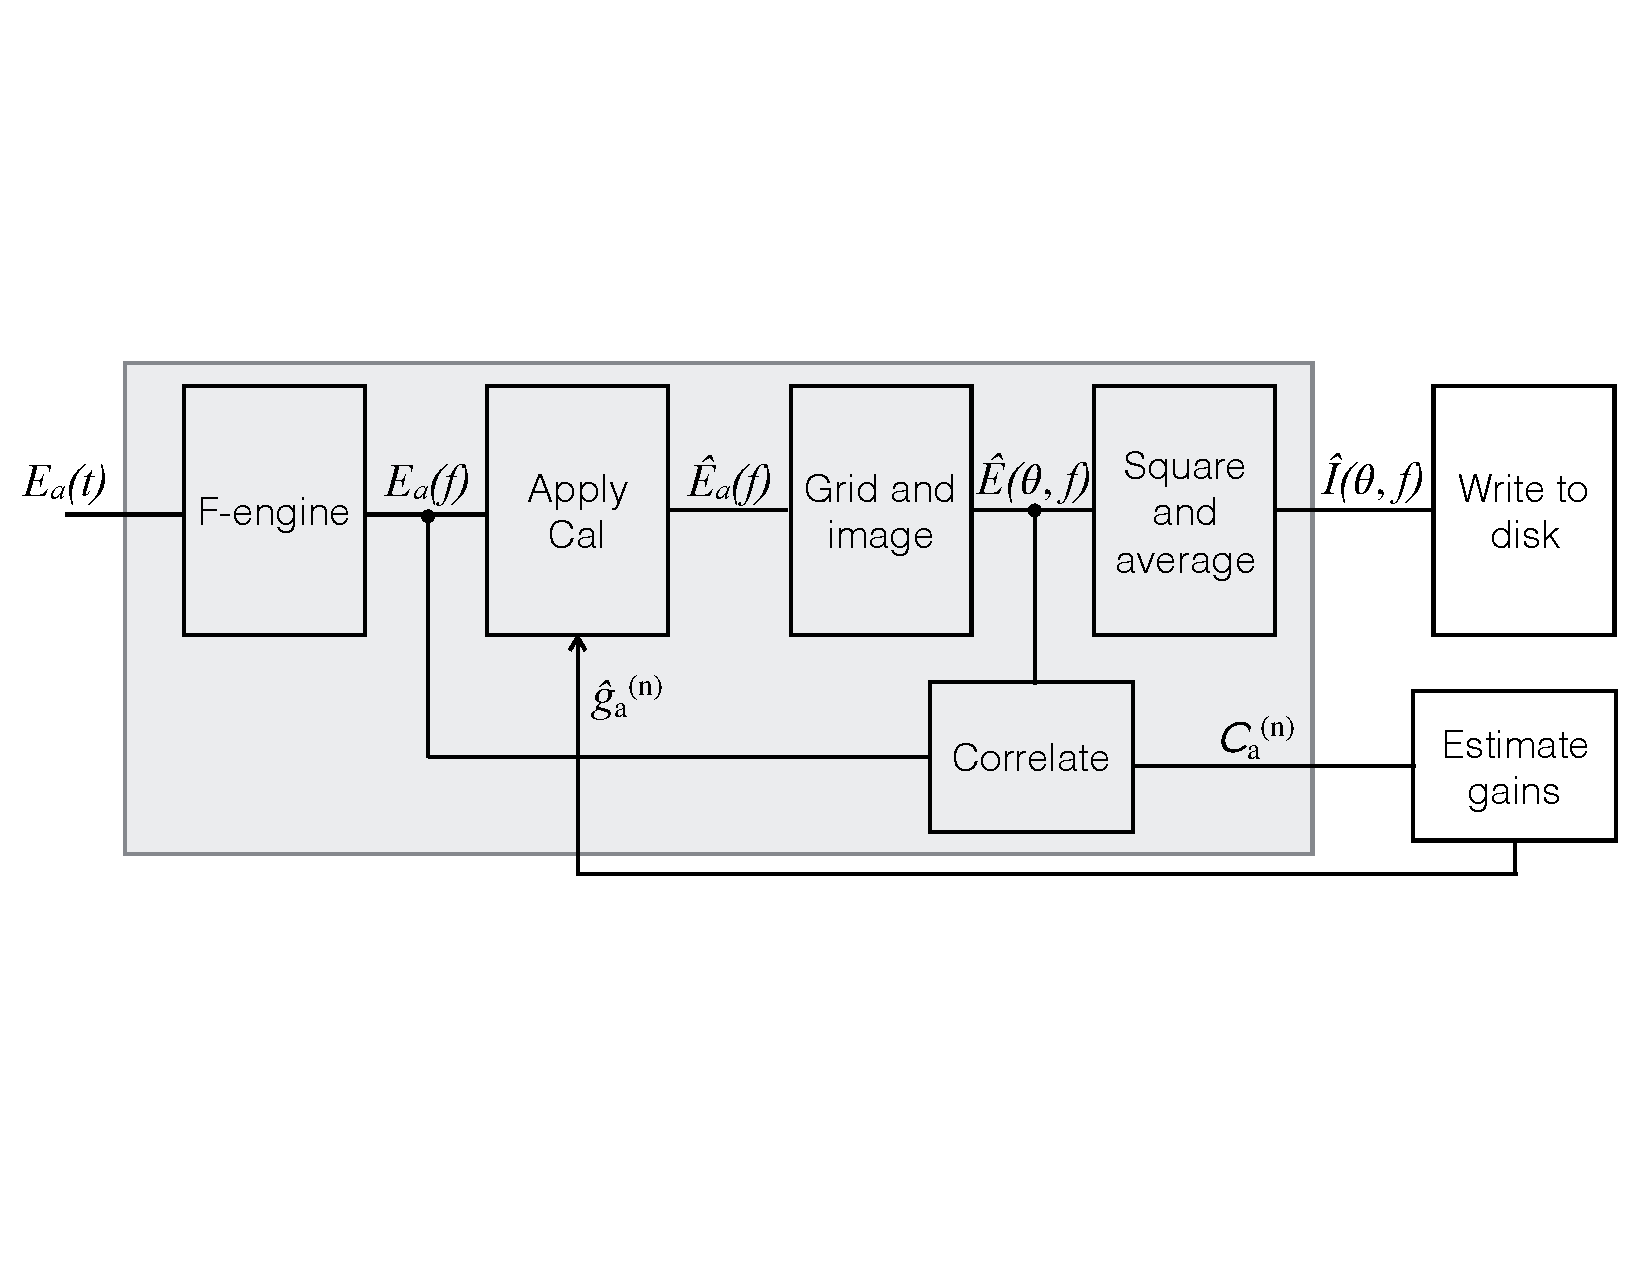
\includegraphics[width=\columnwidth]{figures/schematic.pdf}
\caption{\textcolor{red}{Caption goes here}}
\label{fig:schematic}
\end{center}
\end{figure}

\section{Simulation}\label{sec:sim}
We first demonstrate our calibration method through a controlled simulation. The simulation software used is included in the EPIC package, and we follow a procedure based on that described in \citealt{thy15c}, using the same toy-model sky with 10 point sources of flux density 10 Jy at random location. We assume perfect knowledge of the sky to build our model visibilities.

We use 64 frequency channels each 40 kHz, and each timeseries is 25~$\mu$s long. However, because each channel is independent in the calibration loop we only show the central channel here. Using the MWA array layout \citep{bea12}, we select the inner 51 antennas within a square bounding box of 150~m. The antenna voltage pattern used is a 4.4~m square tophat on the ground.

In order to show our ability to recover unknown complex antenna gains, we create a set of random numbers with amplitude $1\pm0.25$, and completely random phase. These are our ``true gains", and we apply them to the frequency-domain simulated antenna electric fields as in equation~\ref{eq:apply_gain}. Our analysis is blind to these values until the end of the process to check accuracy. We start with an initial guess of unity gains.

We next process \caliter~time stamps, creating both a short-term integrated image and \Cna[0] correlations. Unless otherwise specified, the software automatically selects the brightest source in the sky model to choose the correlation pixel. We use our correlation values to update the gains. We found that simply using equation~\ref{eq:cal_solution} resulted in large oscillations in the solutions, which eventually converged. To mitigate this we introduce a tunable damping factor, $0< \damp \leq 1$, which is used to attenuate the gain update, effectively giving the solutions memory of previous iterations. Through experimentation we found $\Delta=0.65$ resulted in the quickest convergence for this simulation.

We continue the calibration loop by updating our gain estimates, dividing the data by the gains, forming images and \Cna correlations to form the next estimate. This process was repeated \itr~times. In figure~\ref{fig:before_image} we show the integrated image created using our initial guess gains and the first \caliter~time steps. Because the gain phases were completely random the image is

\section{Application to LWA data}\label{sec:data}
Reference for Cyg-A: \citealt{coh07}. Ref for Cas-A: \citealt{kas07}.
Apply to LWA data.

\section{Noise analysis}\label{sec:noise}

Connect to either cramer-rao or FX solutions in some way

Assume we did form visibilities with some integration time. Assuming the noise on each visibility, $\sigma_{ab}$, is independent, we can write the likelihood function of measuring $V_{ab}$ given the true value, the gains, and the noise.
\begin{equation}
\mathcal{L}(V_{ab};\mathbf{g}) = \frac{1}{2\pi \sigma_{ab}^2}\exp\left[-\frac{\left|V_{ab} - g_a g_b^* V_{ab}^T\right|^2}{2\sigma_{ab}^2}\right]
\end{equation}
Then the likelihood of the set of all visibilities will be,
\begin{equation}
\mathcal{L}(\mathbf{V};\mathbf{g}) = \prod_a \prod_{b > a} \mathcal{L}(V_{ab};\mathbf{g})
\end{equation}
The Fischer information matrix for the set of gain parameters is
\begin{equation}
\mathbf{F}^g_{ij} = \left<\left. \frac{\partial \ln \mathcal{L}(\mathbf{V};\mathbf{g})}{\partial g_i} \frac{\partial \ln \mathcal{L}(\mathbf{V};\mathbf{g})}{\partial g_j}\right|_\mathbf{g}\right>.
\end{equation}
We next evaluate the derivate of the log-likelihood.
\begin{equation}
\frac{\partial \ln \mathcal{L}(\mathbf{V};\mathbf{g})}{\partial g_i} = 
\sum_{a \ne i} \frac{g_a^* V_{ai}^{T*} (V_{ai} - g_a g_i^* V_{ai}^T)}{2 \sigma_{ai}^2}
\end{equation}

\textcolor{red}{This part of the argument needs serious work!} In order to find the Cram\'er-Rao lower bound on the variance of the complex parameter, $g_i$, we consider the term of the Fischer matrix where the first derivative is taken with respect to $g_i$, and the second with $g_i^*$. The result is
\begin{align}
\mathbf{F}^g_{ii} = & \left<\left[ \sum_{a \ne i} \frac{g_a^* V_{ai}^{T*} (V_{ai} - g_a g_i^* V_{ai}^T)}{2 \sigma_{ai}^2} \right] \right. \times \nonumber \\
& \left. \left[ \sum_{b \ne i} \frac{g_b V_{bi}^{T} (V_{bi}^* - g_b^* g_i V_{bi}^{T*})}{2 \sigma_{bi}^2} \right] \right> \nonumber \\
= &\sum_{a\ne i} \sum_{b \ne i} \frac{g_a^* g_b V_{ai}^{T*} V_{bi}^T}{4 \sigma_{ai}^2 \sigma_{bi}^2} \left< V_{ai}V_{bi}^* - g_i g_b^* V_{ai}V_{bi}^{T*}\nonumber \right.\\
&\left. - g_a g_i^* V_{ai}^T V_{bi}^* + g_a g_b^* |g_i|^2 V_{ai}^T V_{bi}^{T*}\right>
\label{eq:Fischer_before_expect}
\end{align}

The expected values are easy to evaluate. Each visibility will average to the ``true" value times the respective gains. The term with two visibilities will include a noise term.
\begin{equation}
\left<V_{ai}V_{bi}^*\right> = |g_i|^2 g_a g_b^* V_{ai}^T V_{bi}^{T*} + \sigma_{ai}^2 \delta_{ab}
\end{equation}
Here $\delta_{ab}$ is the Kronecker delta selecting the term where $a=b$ and the noise correlates. Plugging in the expectation values, equation \ref{eq:Fischer_before_expect} simplifies greatly to
\begin{equation}
\mathbf{F}^g_{ii} = \sum_{a \ne i} \frac{\left|g_a V_{ia}^T \right|^2}{4\sigma_{ai}^2}
\end{equation}

Finally we relate our result to the theoretical best uncertainty we can place on our unknown gain parameter using the Cram\'er-Rao lower bound.
\begin{equation}\label{eq:cramer_rao}
\sigma_{g_i}^2 \ge \left[ \mathbf{F}^g_{ii} \right]^{-1} = \left[ \sum_{a \ne i} \frac{\left|g_a V_{ia}^T \right|^2}{4\sigma_{ai}^2} \right]^{-1}
\end{equation}

\section{Discussion}\label{sec:discussion}

\section*{Acknowledgements}
This work has been supported by the National Science Foundation through award AST-1206552.


%%%%%%%%%%%%%%%%%%%% REFERENCES %%%%%%%%%%%%%%%%%%

% The best way to enter references is to use BibTeX:

\bibliographystyle{../mnras}
\bibliography{../epic} % if your bibtex file is called example.bib



%%%%%%%%%%%%%%%%% APPENDICES %%%%%%%%%%%%%%%%%%%%%

\appendix

\section{Some extra material}

If you want to present additional material which would interrupt the flow of the main paper,
it can be placed in an Appendix which appears after the list of references.

%%%%%%%%%%%%%%%%%%%%%%%%%%%%%%%%%%%%%%%%%%%%%%%%%%


% Don't change these lines
\bsp	% typesetting comment
\label{lastpage}
\end{document}

% End of mnras_template.tex